\documentclass[10pt]{article}
\usepackage[polish]{babel}
\usepackage[utf8]{inputenc}
\usepackage[T1]{fontenc}
\usepackage{graphicx}
\usepackage[export]{adjustbox}
\graphicspath{ {./images/} }
\usepackage{amsmath}
\usepackage{amsfonts}
\usepackage{amssymb}
\usepackage[version=4]{mhchem}
\usepackage{stmaryrd}

\title{Zestaw 2. }

\author{}
\date{}


\begin{document}
\maketitle
\begin{center}

\includegraphics[max width=\textwidth]{2024_11_21_2f6840cbb6136169e919g-1(1)}
\end{center}

\section*{GIMNAZJUM}
\begin{enumerate}
  \item Znajdź najmniejszą liczbę zakończoną cyfrą 6 o tej własności, że przeniesienie tej cyfry na początek da nam liczbę cztery razy większą od wyjściowej.
  \item W pewnym sklepie 16 gum do żucia kosztuje dokładnie tyle złotych, ile gum do żucia można kupić za jedną złotówkę. Ile groszy kosztuje jedna guma do żucia?
  \item W trójkącie równobocznym ABC poprowadzono wysokość BD i na przedłużeniu wysokości odłożono punkt K taki, że \(|\mathrm{BK}|=|\mathrm{AC}|\). Punkt K połączono z punktami A i C. Jaką miarę ma kąt AKC?
\end{enumerate}

\section*{LICEUM}
\begin{enumerate}
  \item Wykaż, że jeżeli \(x+y+z=0\), to \(x^{3}+y^{3}+z^{3}=3 x y z\).
  \item Dany jest czworościan \(A B C D\), w którym \(|A B|=5,|C D|=3\) oraz \(\angle A C B=\angle A D B=90^{\circ}\). Znajdź długość odcinka łączącego środki krawędzi AB i CD.\\
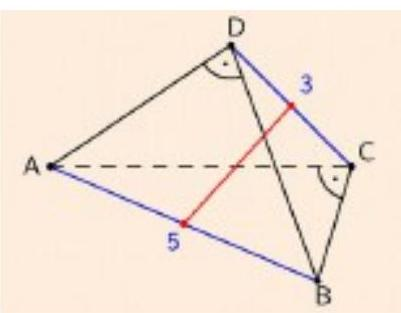
\includegraphics[max width=\textwidth, center]{2024_11_21_2f6840cbb6136169e919g-1}
  \item Oblicz, ile dzielników większych od 13 ma liczba 13! (czyli iloczyn wszystkich liczb naturalnych od 1 do 13).
\end{enumerate}

\end{document}